\documentclass[]{article}
\usepackage{lmodern}
\usepackage{amssymb,amsmath}
\usepackage{ifxetex,ifluatex}
\usepackage{fixltx2e} % provides \textsubscript
\ifnum 0\ifxetex 1\fi\ifluatex 1\fi=0 % if pdftex
  \usepackage[T1]{fontenc}
  \usepackage[utf8]{inputenc}
\else % if luatex or xelatex
  \ifxetex
    \usepackage{mathspec}
  \else
    \usepackage{fontspec}
  \fi
  \defaultfontfeatures{Ligatures=TeX,Scale=MatchLowercase}
\fi
% use upquote if available, for straight quotes in verbatim environments
\IfFileExists{upquote.sty}{\usepackage{upquote}}{}
% use microtype if available
\IfFileExists{microtype.sty}{%
\usepackage{microtype}
\UseMicrotypeSet[protrusion]{basicmath} % disable protrusion for tt fonts
}{}
\usepackage[margin=1in]{geometry}
\usepackage{hyperref}
\hypersetup{unicode=true,
            pdftitle={Trabajo Práctico Final - Estadística Actuarial (751-1)},
            pdfauthor={Zajdenberg, Dana Rebeca (892.786); Barrales Agosti, Julián Guido (889.901); Cohen Falah, Iván Nahuel (890.693); Lopatka, Lucas Eitán (889.524); Ignacio Borovsky (891.119)},
            pdfborder={0 0 0},
            breaklinks=true}
\urlstyle{same}  % don't use monospace font for urls
\usepackage{color}
\usepackage{fancyvrb}
\newcommand{\VerbBar}{|}
\newcommand{\VERB}{\Verb[commandchars=\\\{\}]}
\DefineVerbatimEnvironment{Highlighting}{Verbatim}{commandchars=\\\{\}}
% Add ',fontsize=\small' for more characters per line
\usepackage{framed}
\definecolor{shadecolor}{RGB}{248,248,248}
\newenvironment{Shaded}{\begin{snugshade}}{\end{snugshade}}
\newcommand{\AlertTok}[1]{\textcolor[rgb]{0.94,0.16,0.16}{#1}}
\newcommand{\AnnotationTok}[1]{\textcolor[rgb]{0.56,0.35,0.01}{\textbf{\textit{#1}}}}
\newcommand{\AttributeTok}[1]{\textcolor[rgb]{0.77,0.63,0.00}{#1}}
\newcommand{\BaseNTok}[1]{\textcolor[rgb]{0.00,0.00,0.81}{#1}}
\newcommand{\BuiltInTok}[1]{#1}
\newcommand{\CharTok}[1]{\textcolor[rgb]{0.31,0.60,0.02}{#1}}
\newcommand{\CommentTok}[1]{\textcolor[rgb]{0.56,0.35,0.01}{\textit{#1}}}
\newcommand{\CommentVarTok}[1]{\textcolor[rgb]{0.56,0.35,0.01}{\textbf{\textit{#1}}}}
\newcommand{\ConstantTok}[1]{\textcolor[rgb]{0.00,0.00,0.00}{#1}}
\newcommand{\ControlFlowTok}[1]{\textcolor[rgb]{0.13,0.29,0.53}{\textbf{#1}}}
\newcommand{\DataTypeTok}[1]{\textcolor[rgb]{0.13,0.29,0.53}{#1}}
\newcommand{\DecValTok}[1]{\textcolor[rgb]{0.00,0.00,0.81}{#1}}
\newcommand{\DocumentationTok}[1]{\textcolor[rgb]{0.56,0.35,0.01}{\textbf{\textit{#1}}}}
\newcommand{\ErrorTok}[1]{\textcolor[rgb]{0.64,0.00,0.00}{\textbf{#1}}}
\newcommand{\ExtensionTok}[1]{#1}
\newcommand{\FloatTok}[1]{\textcolor[rgb]{0.00,0.00,0.81}{#1}}
\newcommand{\FunctionTok}[1]{\textcolor[rgb]{0.00,0.00,0.00}{#1}}
\newcommand{\ImportTok}[1]{#1}
\newcommand{\InformationTok}[1]{\textcolor[rgb]{0.56,0.35,0.01}{\textbf{\textit{#1}}}}
\newcommand{\KeywordTok}[1]{\textcolor[rgb]{0.13,0.29,0.53}{\textbf{#1}}}
\newcommand{\NormalTok}[1]{#1}
\newcommand{\OperatorTok}[1]{\textcolor[rgb]{0.81,0.36,0.00}{\textbf{#1}}}
\newcommand{\OtherTok}[1]{\textcolor[rgb]{0.56,0.35,0.01}{#1}}
\newcommand{\PreprocessorTok}[1]{\textcolor[rgb]{0.56,0.35,0.01}{\textit{#1}}}
\newcommand{\RegionMarkerTok}[1]{#1}
\newcommand{\SpecialCharTok}[1]{\textcolor[rgb]{0.00,0.00,0.00}{#1}}
\newcommand{\SpecialStringTok}[1]{\textcolor[rgb]{0.31,0.60,0.02}{#1}}
\newcommand{\StringTok}[1]{\textcolor[rgb]{0.31,0.60,0.02}{#1}}
\newcommand{\VariableTok}[1]{\textcolor[rgb]{0.00,0.00,0.00}{#1}}
\newcommand{\VerbatimStringTok}[1]{\textcolor[rgb]{0.31,0.60,0.02}{#1}}
\newcommand{\WarningTok}[1]{\textcolor[rgb]{0.56,0.35,0.01}{\textbf{\textit{#1}}}}
\usepackage{longtable,booktabs}
\usepackage{graphicx,grffile}
\makeatletter
\def\maxwidth{\ifdim\Gin@nat@width>\linewidth\linewidth\else\Gin@nat@width\fi}
\def\maxheight{\ifdim\Gin@nat@height>\textheight\textheight\else\Gin@nat@height\fi}
\makeatother
% Scale images if necessary, so that they will not overflow the page
% margins by default, and it is still possible to overwrite the defaults
% using explicit options in \includegraphics[width, height, ...]{}
\setkeys{Gin}{width=\maxwidth,height=\maxheight,keepaspectratio}
\setlength{\emergencystretch}{3em}  % prevent overfull lines
\providecommand{\tightlist}{%
  \setlength{\itemsep}{0pt}\setlength{\parskip}{0pt}}
\setcounter{secnumdepth}{0}
% Redefines (sub)paragraphs to behave more like sections
\ifx\paragraph\undefined\else
\let\oldparagraph\paragraph
\renewcommand{\paragraph}[1]{\oldparagraph{#1}\mbox{}}
\fi
\ifx\subparagraph\undefined\else
\let\oldsubparagraph\subparagraph
\renewcommand{\subparagraph}[1]{\oldsubparagraph{#1}\mbox{}}
\fi

%%% Use protect on footnotes to avoid problems with footnotes in titles
\let\rmarkdownfootnote\footnote%
\def\footnote{\protect\rmarkdownfootnote}

%%% Change title format to be more compact
\usepackage{titling}

% Create subtitle command for use in maketitle
\providecommand{\subtitle}[1]{
  \posttitle{
    \begin{center}\large#1\end{center}
    }
}

\setlength{\droptitle}{-2em}

  \title{Trabajo Práctico Final - Estadística Actuarial (751-1)}
    \pretitle{\vspace{\droptitle}\centering\huge}
  \posttitle{\par}
    \author{Zajdenberg, Dana Rebeca (892.786) \\ Barrales Agosti, Julián Guido (889.901) \\ Cohen Falah, Iván Nahuel (890.693) \\ Lopatka, Lucas Eitán (889.524) \\ Ignacio Borovsky (891.119)}
    \preauthor{\centering\large\emph}
  \postauthor{\par}
    \date{}
    \predate{}\postdate{}
  

\begin{document}
\maketitle

\hypertarget{introduccion}{%
\section{Introducción}\label{introduccion}}

~ ~ ~En el presente trabajo se analizarán dos series temporales
correspondientes a dos activos financieros distintos, otorgadas por el
cuerpo docente. A lo largo del mismo se empleará la metodología de
Box-Jenkins, utilizando los conceptos vistos en clase y el programa
R-Studio.

\begin{Shaded}
\begin{Highlighting}[]
\KeywordTok{library}\NormalTok{(moments)}
\KeywordTok{library}\NormalTok{(tseries)}
\KeywordTok{library}\NormalTok{(urca)}
\KeywordTok{library}\NormalTok{(forecast)}
\KeywordTok{library}\NormalTok{(nortest)}
\end{Highlighting}
\end{Shaded}

\begin{longtable}[]{@{}ll@{}}
\toprule
& x\tabularnewline
\midrule
\endhead
Minimo & -5.1431274\tabularnewline
Maximo & 3.2786112\tabularnewline
Percentil 0.25 & -1.2897040\tabularnewline
Mediana & -0.3684681\tabularnewline
Percentil 0.75 & 0.7949836\tabularnewline
Coef Asimetria & -0.2597790\tabularnewline
Coef Curtosis & 3.2940126\tabularnewline
Promedio & -0.3189307\tabularnewline
Varianza & 2.4864574\tabularnewline
Desvio & 1.5768505\tabularnewline
\bottomrule
\end{longtable}

\#\#\#Fase de identificación

~Se grafica la serie para una primera impresión

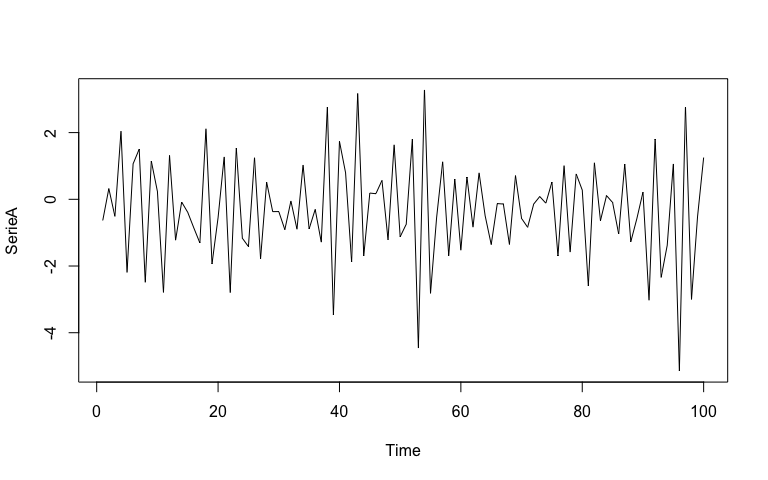
\includegraphics{Script-TPR_files/figure-latex/unnamed-chunk-3-1.pdf}
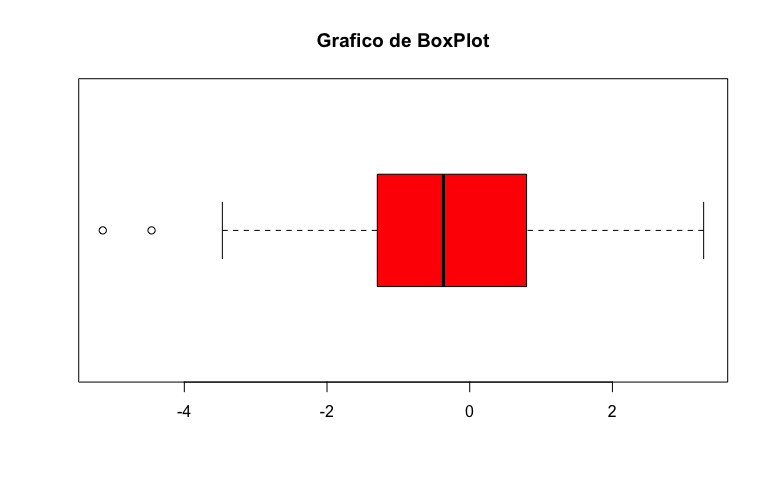
\includegraphics{Script-TPR_files/figure-latex/unnamed-chunk-3-2.pdf}

~El gráfico permite observar una reversion a la media (posiblemente
cero). Se ve que ocurre con la FAC y FACP estimada,

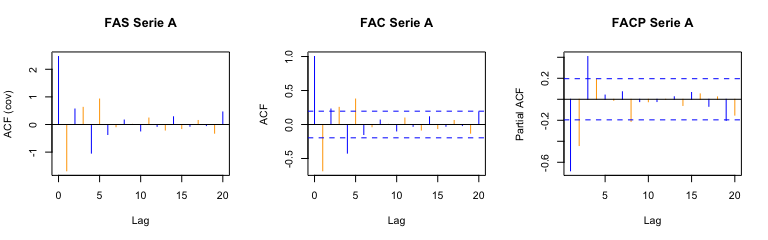
\includegraphics{Script-TPR_files/figure-latex/unnamed-chunk-4-1.pdf}

~ El grafico de la FAC muestra un decrecimiento sinusoidal. Con el
objetivo de determinar la existencia o no de raíces unitarias se efectúa
los tests de Dickey-Fuller.

~Los valores de Tau empíricos para cada modelo son:

\begin{longtable}[]{@{}lr@{}}
\toprule
& x\tabularnewline
\midrule
\endhead
None & -1.493122\tabularnewline
Con Drift & -2.915783\tabularnewline
Con Trend & -3.133971\tabularnewline
\bottomrule
\end{longtable}

~Y los respectivos valores criticos de Tau son

\begin{longtable}[]{@{}lrrr@{}}
\toprule
& 1pct & 5pct & 10pct\tabularnewline
\midrule
\endhead
None & -2.60 & -1.95 & -1.61\tabularnewline
Con Drift & -3.51 & -2.89 & -2.58\tabularnewline
Con Trend & -4.04 & -3.45 & -3.15\tabularnewline
\bottomrule
\end{longtable}

~Por lo tanto se puede afirmar con un nivel de significatividad
aproximado a 5\% que la serie es no estacionaria para todos los modelos.

\#\#Fase de estimacion

~A continuacion, se evaluaron todas las posibles combinaciones de
modelos ARIMA (p,d,q) con p, d y q entre cero y tres con el fin de
seleccionar aquel que mejor ajusta en base a los criterios de
informacion vistos en clase.

\begin{verbatim}
## [1] "Para la serie A, el menor AIC fue de 271.656460053011 para el modelo ARIMA(3, 0, 1)"
\end{verbatim}

\begin{verbatim}
## [1] "Para la serie A, el menor BIC fue de 282.056862231562 para el modelo ARIMA(2, 1, 1)"
\end{verbatim}

~El modelo que mejor se ajusta segun el criterio BIC es un ARIMA (2,1,1)

\begin{Shaded}
\begin{Highlighting}[]
\NormalTok{ModeloA<-}\KeywordTok{arima}\NormalTok{(SerieA, }\DataTypeTok{order=}\KeywordTok{c}\NormalTok{(}\DecValTok{2}\NormalTok{,}\DecValTok{1}\NormalTok{,}\DecValTok{1}\NormalTok{))}
\end{Highlighting}
\end{Shaded}

\[y_t=-1.2741y_{t-1}-0.7230y_{t-1}+0.6280\epsilon_{t-1}\] \#\#Fase de
validación

~Se demuestra primero que los coeficientes del modelo estimado son
significativos. Para esto es utilizada una función que devuelve un
mensaje

\begin{Shaded}
\begin{Highlighting}[]
\NormalTok{TestT<-}\ControlFlowTok{function}\NormalTok{(modelo)\{}
  \ControlFlowTok{for}\NormalTok{(i }\ControlFlowTok{in} \DecValTok{1}\OperatorTok{:}\KeywordTok{length}\NormalTok{(modelo}\OperatorTok{$}\NormalTok{coef)) \{}
\NormalTok{      a=}\KeywordTok{abs}\NormalTok{(modelo}\OperatorTok{$}\NormalTok{coef[i]}\OperatorTok{/}\KeywordTok{sqrt}\NormalTok{(modelo}\OperatorTok{$}\NormalTok{var.coef[i,i]))}
      \ControlFlowTok{if}\NormalTok{(a}\OperatorTok{>=}\DecValTok{2}\NormalTok{) \{}
        \KeywordTok{print}\NormalTok{(}\KeywordTok{paste}\NormalTok{(}\StringTok{"El coeficiente"}\NormalTok{,}\KeywordTok{names}\NormalTok{(modelo}\OperatorTok{$}\NormalTok{coef[i]),}\StringTok{"es un parametro significativo"}\NormalTok{))}
\NormalTok{      \} }\ControlFlowTok{else}\NormalTok{ \{}
        \KeywordTok{paste}\NormalTok{(}\KeywordTok{print}\NormalTok{(}\StringTok{"no es significativo"}\NormalTok{))}
\NormalTok{      \}}
\NormalTok{  \}}
\NormalTok{\}}
\end{Highlighting}
\end{Shaded}

~Se ingresa el modelo estimado como input y el codigo devuelve

\begin{Shaded}
\begin{Highlighting}[]
\KeywordTok{TestT}\NormalTok{(ModeloA)}
\end{Highlighting}
\end{Shaded}

\begin{verbatim}
## [1] "El coeficiente ar1 es un parametro significativo"
## [1] "El coeficiente ar2 es un parametro significativo"
## [1] "El coeficiente ma1 es un parametro significativo"
\end{verbatim}

~El siguiente paso es que el modelo cumpla con las condiciones de
estacionariedad e invertibilidad.

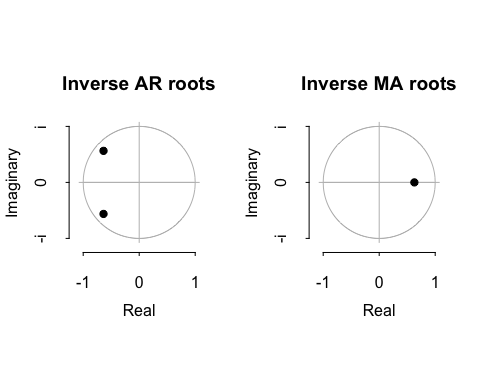
\includegraphics{Script-TPR_files/figure-latex/unnamed-chunk-12-1.pdf}

~Las raices caen dentro del circulo unidad\\
\hspace*{0.333em} ~Ahora se analiza la normalidad de los residuos. Para
ello se realiza un gráfico de \emph{qqnorm} que compara los cuantiles
teóricos de la distribución normal con los de los residuos de la serie.

\begin{Shaded}
\begin{Highlighting}[]
\KeywordTok{qqnorm}\NormalTok{(ModeloA}\OperatorTok{$}\NormalTok{residuals)}
\KeywordTok{qqline}\NormalTok{(ModeloA}\OperatorTok{$}\NormalTok{residuals)}
\end{Highlighting}
\end{Shaded}

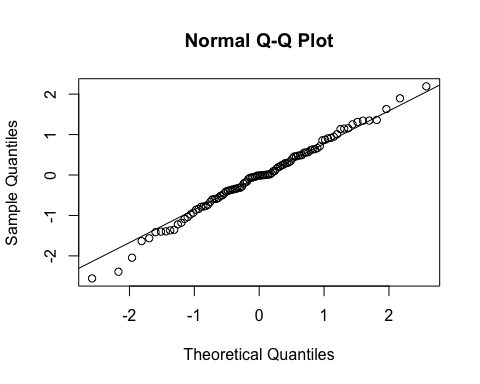
\includegraphics{Script-TPR_files/figure-latex/unnamed-chunk-13-1.pdf}

~Para complementar el \textbf{analisis de normalidad} es realizado un
test de Jarque Bera

\begin{Shaded}
\begin{Highlighting}[]
\KeywordTok{jarque.bera.test}\NormalTok{(ModeloA}\OperatorTok{$}\NormalTok{residuals)}
\end{Highlighting}
\end{Shaded}

\begin{verbatim}
## 
##  Jarque Bera Test
## 
## data:  ModeloA$residuals
## X-squared = 0.84112, df = 2, p-value = 0.6567
\end{verbatim}

~ Como el \emph{p-value} es 0.6567 y es mayor a un \(\alpha\) de 0.1 no
rechaza la hipotesis nula de normalidad de los reisudos. ~ ~Por ultimo,
la \textbf{incorrelacion de los residuos} es analizada. Se ejecuta el
test de Ljung-Box y se obtiene,

\begin{Shaded}
\begin{Highlighting}[]
\KeywordTok{Box.test}\NormalTok{(ModeloA}\OperatorTok{$}\NormalTok{residuals,}\DataTypeTok{lag=}\DecValTok{5}\NormalTok{,}\DataTypeTok{type =}\StringTok{"Ljung-Box"}\NormalTok{,}\DataTypeTok{fitdf =} \DecValTok{3}\NormalTok{)}
\end{Highlighting}
\end{Shaded}

\begin{verbatim}
## 
##  Box-Ljung test
## 
## data:  ModeloA$residuals
## X-squared = 2.0956, df = 2, p-value = 0.3507
\end{verbatim}

\begin{Shaded}
\begin{Highlighting}[]
\KeywordTok{Box.test}\NormalTok{(ModeloA}\OperatorTok{$}\NormalTok{residuals,}\DataTypeTok{lag=}\DecValTok{7}\NormalTok{,}\DataTypeTok{type =}\StringTok{"Ljung-Box"}\NormalTok{,}\DataTypeTok{fitdf =} \DecValTok{3}\NormalTok{)}
\end{Highlighting}
\end{Shaded}

\begin{verbatim}
## 
##  Box-Ljung test
## 
## data:  ModeloA$residuals
## X-squared = 3.7459, df = 4, p-value = 0.4415
\end{verbatim}

\begin{Shaded}
\begin{Highlighting}[]
\KeywordTok{Box.test}\NormalTok{(ModeloA}\OperatorTok{$}\NormalTok{residuals,}\DataTypeTok{lag=}\DecValTok{9}\NormalTok{,}\DataTypeTok{type =}\StringTok{"Ljung-Box"}\NormalTok{,}\DataTypeTok{fitdf =} \DecValTok{3}\NormalTok{)}
\end{Highlighting}
\end{Shaded}

\begin{verbatim}
## 
##  Box-Ljung test
## 
## data:  ModeloA$residuals
## X-squared = 6.42, df = 6, p-value = 0.3778
\end{verbatim}

~Entonces, con un \(\alpha\) de 0.1, se puede afirmar que los residuos
no estan correlacionados para valores propios desfasados en el dominio
del tiempo.

\hypertarget{fase-de-prediccion}{%
\subsection{Fase de Predicción}\label{fase-de-prediccion}}

~La predicción finalmente para un horizonte de diez periodos y con un
nivel de confianza al 95\% es,

\begin{Shaded}
\begin{Highlighting}[]
\KeywordTok{par}\NormalTok{(}\DataTypeTok{mfrow=}\KeywordTok{c}\NormalTok{(}\DecValTok{2}\NormalTok{,}\DecValTok{2}\NormalTok{))}
\KeywordTok{plot}\NormalTok{(}\KeywordTok{forecast}\NormalTok{(ModeloA, }\DecValTok{1}\NormalTok{,}\DataTypeTok{level=}\DecValTok{95}\NormalTok{), }\DataTypeTok{main=}\StringTok{"Prediccion 1 periodo"}\NormalTok{)}
\KeywordTok{plot}\NormalTok{(}\KeywordTok{forecast}\NormalTok{(ModeloA, }\DecValTok{2}\NormalTok{,}\DataTypeTok{level=}\DecValTok{95}\NormalTok{), }\DataTypeTok{main=}\StringTok{"Prediccion 2 periodos"}\NormalTok{)}
\KeywordTok{plot}\NormalTok{(}\KeywordTok{forecast}\NormalTok{(ModeloA, }\DecValTok{3}\NormalTok{,}\DataTypeTok{level=}\DecValTok{95}\NormalTok{), }\DataTypeTok{main=}\StringTok{"Prediccion 3 periodos"}\NormalTok{)}
\KeywordTok{plot}\NormalTok{(}\KeywordTok{forecast}\NormalTok{(ModeloA, }\DecValTok{20}\NormalTok{,}\DataTypeTok{level=}\DecValTok{95}\NormalTok{), }\DataTypeTok{main=}\StringTok{"Prediccion 20 periodos"}\NormalTok{)}
\end{Highlighting}
\end{Shaded}

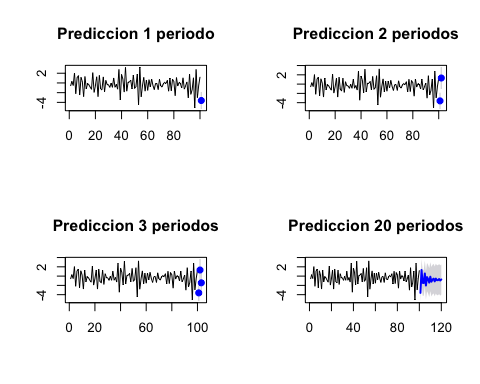
\includegraphics{Script-TPR_files/figure-latex/unnamed-chunk-16-1.pdf}

~Los valores del gráfico son representados en el siguiente cuadro. Se
calcularon los intervalos para el 94\%, 95\% y 99\% de confianza.

\begin{longtable}[]{@{}lllllll@{}}
\caption{Intervalos de confianza para el Modelo A}\tabularnewline
\toprule
Limite inferior 0.99 & Limite inferior 0.95 & Limite inferior 0.94 &
Prediccion & Limite sueprior 0.94 & Limite superior 0.95 & Limite
superior 0.99\tabularnewline
\midrule
\endfirsthead
\toprule
Limite inferior 0.99 & Limite inferior 0.95 & Limite inferior 0.94 &
Prediccion & Limite sueprior 0.94 & Limite superior 0.95 & Limite
superior 0.99\tabularnewline
\midrule
\endhead
-5.926600 & -5.374150 & -5.3031319 & -3.616003 & -1.928873 & -1.857855 &
-1.305405\tabularnewline
-1.798766 & -1.054716 & -0.9590676 & 1.313188 & 3.585444 & 3.681092 &
4.425142\tabularnewline
-5.064972 & -4.199999 & -4.0888049 & -1.447258 & 1.194290 & 1.305483 &
2.170457\tabularnewline
-5.002368 & -3.979625 & -3.8481501 & -0.724792 & 2.398566 & 2.530041 &
3.552784\tabularnewline
\bottomrule
\end{longtable}

~Efectuado el analisis, se procede a exportar los datos en formato CSV

\begin{Shaded}
\begin{Highlighting}[]
\NormalTok{Serie_estimadaA<-}\KeywordTok{c}\NormalTok{(SerieA,}\KeywordTok{forecast}\NormalTok{(ModeloA, }\DecValTok{20}\NormalTok{, }\DataTypeTok{level=}\DecValTok{95}\NormalTok{)}\OperatorTok{$}\NormalTok{mean)}
\KeywordTok{data.frame}\NormalTok{(x)}
\KeywordTok{write.csv}\NormalTok{(Serie_estimadaA,}\StringTok{"/Users/iborovsky/Desktop/TPR/SerieEstimadaA.csv"}\NormalTok{)}
\end{Highlighting}
\end{Shaded}

\hypertarget{analisis-de-la-serie-numero-dos}{%
\subsection{Análisis de la serie numero
dos}\label{analisis-de-la-serie-numero-dos}}

~Ahora se repite el análisis para la siguiente serie. En principio, se
describe la serie.

\begin{longtable}[]{@{}ll@{}}
\toprule
& x\tabularnewline
\midrule
\endhead
Minimo & -2.4547686\tabularnewline
Maximo & 3.6702532\tabularnewline
Percentil 0.25 & -0.8725365\tabularnewline
Mediana & -0.1852117\tabularnewline
Percentil 0.75 & 0.5928155\tabularnewline
Coef Asimetria & 0.5265426\tabularnewline
Coef Curtosis & 3.7810109\tabularnewline
Promedio & -0.0849636\tabularnewline
Varianza & 1.1587634\tabularnewline
Desvio & 1.0764587\tabularnewline
\#\#\#Fase de identi & ficacion\tabularnewline
\bottomrule
\end{longtable}

~Se observa el gráfico de la serie

\includegraphics{Script-TPR_files/figure-latex/unnamed-chunk-20-1.pdf}
\includegraphics{Script-TPR_files/figure-latex/unnamed-chunk-20-2.pdf}

~El mismo no permite ver en principio la reversion a la media. Continúa
con la FAC y FACP estimada,

\includegraphics{Script-TPR_files/figure-latex/unnamed-chunk-21-1.pdf}

~A través de la FACP se verifica que decrece lentamente de manera
sinusoidal. Por otro lado, la FAC se anula al primer rezago. Los
gráficos proponen la posibilidad de que sea un proceso de medias moviles
no estacionaro. Para confirmar estas intuiciones son realizados los
correspondientes tests de Dickey-Füller

~Los valores de Tau empíricos para cada modelo son:

\begin{longtable}[]{@{}lr@{}}
\toprule
& x\tabularnewline
\midrule
\endhead
None & -1.884895\tabularnewline
Con Drift & -1.936875\tabularnewline
Con Trend & -3.594724\tabularnewline
\bottomrule
\end{longtable}

~Y los respectivos valores criticos de Tau son

\begin{longtable}[]{@{}lrrr@{}}
\toprule
& 1pct & 5pct & 10pct\tabularnewline
\midrule
\endhead
None & -2.60 & -1.95 & -1.61\tabularnewline
Con Drift & -3.51 & -2.89 & -2.58\tabularnewline
Con Trend & -4.04 & -3.45 & -3.15\tabularnewline
\bottomrule
\end{longtable}

~ Existe evidencia suficiente para que sea razonable no rechazar la
hipótesis nula de estacionariedad para modelos \emph{none} y
\emph{drift}. Sin embargo, se rechaza para un modelo con tendencia.
(Supone un \(\alpha\) del 5\%)

\#\#\#Fase de estimacion

~Se reutiliza el codigo para la seleccion del modelo anterior. El que
mejor se ajusta segun BIC es el modelo ARIMA (0,1,2)

\begin{verbatim}
## [1] "Para la serie B, el menor AIC fue de 274.510249397882 para el modelo ARIMA(0, 1, 2)"
\end{verbatim}

\begin{verbatim}
## [1] "Para la serie B, el menor BIC fue de 282.295608948286 para el modelo ARIMA(0, 1, 2)"
\end{verbatim}

~ Entonces el modelo apropiado es,

\begin{Shaded}
\begin{Highlighting}[]
\NormalTok{ModeloB<-}\KeywordTok{arima}\NormalTok{(SerieB, }\DataTypeTok{order=}\KeywordTok{c}\NormalTok{(}\DecValTok{0}\NormalTok{,}\DecValTok{1}\NormalTok{,}\DecValTok{2}\NormalTok{))}
\end{Highlighting}
\end{Shaded}

\[\hat{y_t}=1.2202\epsilon_{t-1}-0.3677\epsilon_{t-2}\]

\#\#Fase de validacion

~Se verifica que los coeficientes del modelo estimado son
significativos,

\begin{Shaded}
\begin{Highlighting}[]
\KeywordTok{TestT}\NormalTok{(ModeloB)}
\end{Highlighting}
\end{Shaded}

\begin{verbatim}
## [1] "El coeficiente ma1 es un parametro significativo"
## [1] "El coeficiente ma2 es un parametro significativo"
\end{verbatim}

~ la condicion de invertibilidad,

\includegraphics{Script-TPR_files/figure-latex/unnamed-chunk-28-1.pdf}

~Cae dentro del círculo unidad ambas raíces

~Ahora se analiza la normalidad de los residuos. Se repite el gráfico de
\emph{qqnorm}

\includegraphics{Script-TPR_files/figure-latex/unnamed-chunk-29-1.pdf}

~Se observa que los cuantiles teóricos coinciden con los cuantiles de
los residuos.

~Para complementar, el \textbf{analisis de normalidad} se utiliza el
test de Jarque Bera

\begin{verbatim}
## 
##  Jarque Bera Test
## 
## data:  ModeloB$residuals
## X-squared = 0.012999, df = 2, p-value = 0.9935
\end{verbatim}

~Como el \emph{pvalue} es cercano a uno, se tiene cierta certeza de que
los residuos del modelo estimado siguen una distribución normal.

~Respecto de la \textbf{incorrelacion de los residuos}. Se utiliza el
test de Ljung-Box para distintos rezagos.

\begin{verbatim}
## 
##  Box-Ljung test
## 
## data:  ModeloB$residuals
## X-squared = 0.18657, df = 1, p-value = 0.6658
\end{verbatim}

\begin{verbatim}
## 
##  Box-Ljung test
## 
## data:  ModeloB$residuals
## X-squared = 0.7578, df = 3, p-value = 0.8595
\end{verbatim}

\begin{verbatim}
## 
##  Box-Ljung test
## 
## data:  ModeloB$residuals
## X-squared = 2.2051, df = 5, p-value = 0.8201
\end{verbatim}

~Los test de incorrelación para rezagos de 4, 6, y 8 arrojan
respectivamente valores \emph{p} de 0.91, 0.94 y 0.899. Por lo tanto,
hay suficiente evidencia de que los residuos del modelo estan
incorrelacionados para valores defasados.

\#\#Fase de predicción

~Como se remarcó anteriormente, no es correcto predecir a partir de un
modelo de medias móviles. Sin embargo, se ejecuta el código para
observar los resultados.

\includegraphics{Script-TPR_files/figure-latex/unnamed-chunk-32-1.pdf}

~Se vuelcan los resultados en la tabla,

\begin{longtable}[]{@{}lllllll@{}}
\caption{Intervalos de confianza para el Modelo B}\tabularnewline
\toprule
Limite inferior 0.99 & Limite inferior 0.95 & Limite inferior 0.94 &
Prediccion & Limite sueprior 0.94 & Limite superior 0.95 & Limite
superior 0.99\tabularnewline
\midrule
\endfirsthead
\toprule
Limite inferior 0.99 & Limite inferior 0.95 & Limite inferior 0.94 &
Prediccion & Limite sueprior 0.94 & Limite superior 0.95 & Limite
superior 0.99\tabularnewline
\midrule
\endhead
-3.144299 & -2.571402 & -2.497756 & -0.7481834 & 1.001389 & 1.075036 &
1.647932\tabularnewline
-3.015761 & -2.429135 & -2.353723 & -0.5622211 & 1.229281 & 1.304693 &
1.891319\tabularnewline
-3.041058 & -2.448383 & -2.372194 & -0.5622211 & 1.247752 & 1.323941 &
1.916616\tabularnewline
-3.437248 & -2.749847 & -2.661480 & -0.5622211 & 1.537038 & 1.625404 &
2.312806\tabularnewline
\bottomrule
\end{longtable}

~Efectuado el análisis, los datos son exportados en formato CSV.

\begin{Shaded}
\begin{Highlighting}[]
\NormalTok{Serie_extendidaB<-}\KeywordTok{c}\NormalTok{(SerieB,}\KeywordTok{forecast}\NormalTok{(ModeloB, }\DecValTok{20}\NormalTok{, }\DataTypeTok{level=}\DecValTok{95}\NormalTok{)}\OperatorTok{$}\NormalTok{mean)}
\KeywordTok{write.csv}\NormalTok{(Serie_extendidaB,}\StringTok{"/Users/iborovsky/Desktop/TPR/SerieEstimadaB.csv"}\NormalTok{)}
\end{Highlighting}
\end{Shaded}

\begin{center}\rule{0.5\linewidth}{\linethickness}\end{center}

\hypertarget{conclusiones}{%
\section{Conclusiones}\label{conclusiones}}

~ Se realizaron dos análisis, uno por cada serie.\\
\hspace*{0.333em}\\
\hspace*{0.333em} La primer serie resultó no ser estacionaria. Se
modelizó la misma para un ARIMA(2,1,1) donde se verificaron todos los
supuestos vistos en el curso y finalmente concluyó con una predicción
para diez períodos.\\
\hspace*{0.333em} ~ En cuanto a la segunda serie, tampoco pudo
demostrarse su estacionariedad. El modelo indicado fue un ARIMA (0,1,2)
que cumplió con todos los supuestos, tanto los de invertibilidad y como
aquellos correspondientes a los residuos. Su predicción arrojó un
resultado ambiguo por los motivos expresados con anterioridad.

\hypertarget{futuras-investigaciones-y-limitaciones}{%
\section{Futuras investigaciones y
limitaciones}\label{futuras-investigaciones-y-limitaciones}}

~ El análisis efectuado se limitó a los modelos de la familia ARIMA. No
se tomó en cuenta la posibilidad de realizar una diferencación
fraccionaria, ni modelizar la serie en otras familias de modelos para
series de tiempo.\\
\hspace*{0.333em} Por otra parte, se utilizaron los tests vistos y
estudiados en la materia \emph{751-Estadistica Actuarial}. Como se
utilizó Dickey-Fuller para el análisis de raíces unitaras se pudieron
haber utilizado otros tests como el de KPSS o Phillips-Perron.

\begin{center}\rule{0.5\linewidth}{\linethickness}\end{center}

\hypertarget{bibliografia}{%
\section{Bibliografía}\label{bibliografia}}

\begin{itemize}
\tightlist
\item
  \emph{Analisis de series temporales: modelos ARIMA} - Ezequiel Uriel
  Jimenez; Valencia, España, 1985.
\item
  \emph{``Time Series Analysis. Forecasting and Control. Fourth
  edition''} - George E. P. Box, Gwilym M. Jenkins, Gregory C. Reinsel.
\item
  \emph{Acerca de la probabilidad} - Alberto H Landro, 2010.
\end{itemize}

\begin{center}\rule{0.5\linewidth}{\linethickness}\end{center}


\end{document}
